\section{Arquitetura do Cluster}
\label{sec:arquitetura}

A análise foi executada sobre um cluster \textbf{Apache Spark 3.5.0} totalmente
conteinerizado com \texttt{Docker} e orquestrado via \texttt{docker-compose}. Essa
escolha garante um ambiente reprodutível e isolado, no qual cada nó do cluster
corresponde a um contêiner independente, comunicando-se por uma rede dedicada. O
ambiente utiliza \textbf{Python 3.8}, versão padrão da imagem base
\texttt{apache/spark:3.5.0}.

O cluster segue o modelo \textbf{master/worker} (mestre/trabalhador) do Spark Standalone
e é composto pelos seguintes serviços:

\begin{itemize}
  \item \textbf{1 Spark Master} (\texttt{spark-master}): processo coordenador
        responsável por gerenciar os recursos do cluster e escalonar as aplicações.
        Expõe a porta \texttt{7077} para submissão de jobs e a \texttt{8080} para a
        interface web de monitoramento.
  \item \textbf{3 Spark Workers} (\texttt{spark-worker-1}, \texttt{-2} e \texttt{-3}):
        nós trabalhadores que executam efetivamente as tarefas. Cada worker é
        configurado com \texttt{SPARK\_WORKER\_CORES=2} e
        \texttt{SPARK\_WORKER\_MEMORY=4g}, totalizando \textbf{6 cores} e
        \textbf{12\,GB} de memória disponíveis para processamento paralelo.
  \item \textbf{1 History Server} (\texttt{spark-history}): serviço que lê o diretório
        de eventos (\texttt{spark-events}) e disponibiliza, na porta \texttt{18080}, o
        histórico de aplicações já finalizadas, permitindo a análise \textit{post-mortem}
        das DAGs e estágios.
  \item \textbf{1 JupyterLab} (\texttt{jupyter}): ambiente interativo de
        desenvolvimento construído a partir de uma imagem customizada
        (\texttt{Dockerfile.jupyter}), baseada em \texttt{apache/spark:3.5.0} com a
        adição das bibliotecas \texttt{numpy}, \texttt{matplotlib}, \texttt{pandas} e
        \texttt{pyspark==3.5.0}. Atua como \textit{driver} da aplicação, conectando-se
        ao master pela porta \texttt{8888}.
\end{itemize}

Todos os serviços estão conectados a uma rede \textit{bridge} do Docker, denominada
\texttt{spark-network}, que isola o tráfego do cluster e permite que os contêineres se
resolvam entre si por \textit{hostname} (por exemplo, \texttt{spark://spark-master:7077}).
Volumes compartilhados (\texttt{./spark-apps}, \texttt{./spark-data} e
\texttt{./spark-events}) garantem que código, dados de entrada/saída e logs de eventos
sejam visíveis de forma consistente em todos os nós.

\subsection{Trecho do \texttt{docker-compose.yml}}

O Código~\ref{lst:compose} ilustra a definição do \textit{master}, de um \textit{worker}
representativo e da rede \texttt{spark-network}. Os demais workers são análogos, variando
apenas o \textit{hostname} e a porta da interface web.

\begin{lstlisting}[language={},caption={Trecho do \texttt{docker-compose.yml}: master, worker e rede bridge.},label={lst:compose}]
services:
  spark-master:
    build: .
    container_name: spark-master
    hostname: spark-master
    command: /opt/spark/bin/spark-class org.apache.spark.deploy.master.Master
    environment:
      - SPARK_MASTER_HOST=spark-master
      - SPARK_MASTER_PORT=7077
      - SPARK_MASTER_WEBUI_PORT=8080
    ports:
      - "8080:8080"
      - "7077:7077"
    networks:
      - spark-network

  spark-worker-1:
    build: .
    container_name: spark-worker-1
    hostname: spark-worker-1
    command: /opt/spark/bin/spark-class org.apache.spark.deploy.worker.Worker spark://spark-master:7077
    environment:
      - SPARK_WORKER_CORES=2
      - SPARK_WORKER_MEMORY=4g
      - SPARK_WORKER_WEBUI_PORT=8081
    depends_on:
      - spark-master
    networks:
      - spark-network

networks:
  spark-network:
    driver: bridge
\end{lstlisting}

\section{Metodologia de ETL}
\label{sec:etl}

O processo de \textbf{ETL} (\textit{Extract, Transform, Load}) foi responsável por
transformar dados climáticos brutos em um conjunto confiável para análise. A base
principal foi o \texttt{GlobalLandTemperaturesByCity.csv}, complementada pela base de
emissões \texttt{owid-co2-data.csv}. As etapas são detalhadas a seguir.

\subsection{Leitura com inferência de esquema}

A ingestão utilizou \texttt{spark.read.csv} com \texttt{header=True} e
\texttt{inferSchema=True}. A inferência automática faz o Spark amostrar os dados para
deduzir os tipos de cada coluna (datas, \texttt{double}, \texttt{string}), dispensando a
definição manual de um \texttt{StructType} e simplificando o protótipo.

\begin{lstlisting}[caption={Leitura da base de temperaturas com inferência de esquema.},label={lst:leitura}]
df = spark.read.csv(
    "/opt/spark-data/input/GlobalLandTemperaturesByCity.csv",
    header=True,
    inferSchema=True,
)
\end{lstlisting}

\subsection{Remoção de nulos, conversão de datas e limpeza de coordenadas}

Registros sem temperatura média (\texttt{AverageTemperature} nulo) não agregam valor
analítico e foram descartados com \texttt{dropna}. A coluna textual \texttt{dt} foi
convertida para o tipo data com \texttt{to\_date}, e dela extraíram-se as colunas
\texttt{Year} e \texttt{Month} via \texttt{year()} e \texttt{month()}, facilitando os
agrupamentos temporais.

As coordenadas vinham no formato \texttt{"57.05N"} / \texttt{"10.33E"}, misturando número
e ponto cardeal. Para viabilizar o filtro geográfico das zonas tropicais (P4), aplicou-se
\texttt{regexp\_replace} removendo os caracteres \texttt{[NSEW]} e convertendo o resultado
para \texttt{double}. Todas as transformações foram encadeadas de forma declarativa
(\textit{lazy}), construindo o DataFrame \texttt{df\_limpo}.

\begin{lstlisting}[caption={Conversão de datas, remoção de nulos e limpeza de coordenadas.},label={lst:limpeza}]
df_limpo = (
    df.withColumn("dt", to_date(col("dt")))
    .withColumn("Year", year(col("dt")))
    .withColumn("Month", month(col("dt")))
    .dropna(subset=["AverageTemperature"])
    .withColumn(
        "Latitude", regexp_replace(col("Latitude"), "[NSEW]", "").cast("double")
    )
    .withColumn(
        "Longitude", regexp_replace(col("Longitude"), "[NSEW]", "").cast("double")
    )
)
\end{lstlisting}

\subsection{Aplicação de \texttt{cache}}

Como \texttt{df\_limpo} é reutilizado por praticamente todas as perguntas, aplicou-se
\texttt{cache()} logo após a limpeza. Sem isso, cada ação (\texttt{count}, \texttt{show},
agregações) reexecutaria todo o pipeline de leitura e transformação a partir do disco. O
\texttt{cache} materializa o resultado em memória após a primeira ação, e as etapas
subsequentes reaproveitam esses dados. A justificativa quantitativa é detalhada na
Seção~\ref{sec:cache}.

\begin{lstlisting}[caption={Materialização em memória do DataFrame limpo.},label={lst:cache}]
df_limpo.show(5)
# Otimizacao: cache no DataFrame limpo, evitando reprocessar a cada nova acao
df_limpo.cache()
\end{lstlisting}

\subsection{Leitura e limpeza da base de CO\textsubscript{2}}

A base \texttt{owid-co2-data.csv} contém, além de países, diversos \textbf{agregados}
(\texttt{"World"}, \texttt{"Asia (GCP)"}, blocos regionais e grupos de renda como
\texttt{"High-income countries"}). Se mantidos, esses agregados seriam contabilizados em
dobro no \textit{join} com a base de temperaturas (que é granularizada por país),
distorcendo a correlação da P6. Por isso foram explicitamente filtrados com
\texttt{\textasciitilde col("country").isin([...])}. Também se restringiu o período a
\texttt{year >= 1900} e removeram-se linhas sem valor de \texttt{co2}.

\begin{lstlisting}[caption={Filtragem de agregados globais e seleção de colunas da base de CO2.},label={lst:co2}]
df_co2_clean = (
    df_co2.filter(col("year") >= 1900)
    .filter(
        ~col("country").isin(
            [
                "World", "Asia", "Asia (GCP)", "Europe", "Africa",
                "North America", "South America", "Oceania",
                "European Union (27)", "European Union (28)",
                "High-income countries", "Low-income countries",
                "Lower-middle-income countries", "Upper-middle-income countries",
                "OECD (GCP)", "Non-OECD (GCP)",
                # ... demais blocos regionais e grupos de renda
            ]
        )
    )
    .select(
        col("country").alias("Country_CO2"),
        col("year").alias("Year_CO2"),
        col("co2"),
        col("co2_per_capita"),
        col("total_ghg"),
    )
    .dropna(subset=["co2"])
)
\end{lstlisting}

\subsection{Filtro de incerteza via \textit{Window Function}}

O \textit{dataset} traz a coluna \texttt{AverageTemperatureUncertainty}. Para descartar
medições pouco confiáveis, definiu-se uma janela particionada por \texttt{City} e
\texttt{Country} e calculou-se a média histórica de cada cidade
(\texttt{HistAvg}). Uma \textit{Window Function} retorna um valor agregado para
\textbf{cada linha} sem colapsar o DataFrame, o que permite comparar a incerteza de cada
registro com a média histórica da sua própria cidade. Mantiveram-se apenas os registros
cuja incerteza fosse menor ou igual a 10\% dessa média.

\begin{lstlisting}[caption={Definição da janela por cidade e filtro de incerteza relativa.},label={lst:incerteza}]
window_city = Window.partitionBy("City", "Country")

df_limpo_com_histavg = df_limpo.withColumn(
    "HistAvg", avg("AverageTemperature").over(window_city)
)

df_filtrado = df_limpo_com_histavg.filter(
    col("AverageTemperatureUncertainty") <= (0.10 * col("HistAvg"))
)
\end{lstlisting}

\section{Análise de Otimização --- Cache}
\label{sec:cache}

\subsection{O que é \texttt{.cache()} e como funciona}

No Spark, transformações são \textbf{preguiçosas} (\textit{lazy}): apenas constroem um
plano lógico, a DAG. Esse plano só é executado quando uma \textbf{ação} (\texttt{count},
\texttt{show}, \texttt{collect}, escrita) é disparada. Por padrão, o resultado de um
DataFrame \textbf{não é guardado}; cada nova ação reexecuta toda a cadeia desde a leitura
do arquivo.

O método \texttt{.cache()} altera esse comportamento. Internamente ele marca o DataFrame
com o nível de armazenamento \texttt{MEMORY\_AND\_DISK}: na primeira ação subsequente, o
Spark calcula o resultado e o \textbf{persiste em memória} nos executores (transbordando
para disco se faltar RAM). A partir daí, as próximas ações leem diretamente dessas
partições materializadas, eliminando a releitura de disco e o reprocessamento das
transformações.

\subsection{Por que foi aplicado em \texttt{df\_limpo}}

\texttt{df\_limpo} é o tronco comum de todo o pipeline: a partir dele derivam o filtro de
incerteza, a análise por década (P1), o ranking de risco (P3), as zonas tropicais (P4) e
demais perguntas. Sem cache, cada uma dessas ramificações refaria a leitura do CSV e toda
a limpeza. Persistindo \texttt{df\_limpo}, paga-se o custo da limpeza \textbf{uma única
vez} e reaproveita-se o resultado em todas as análises.

\subsection{Comparativo de desempenho}

Para mensurar o ganho de forma controlada, instrumentou-se o tempo de uma mesma ação
(\texttt{count}) em dois cenários: a \textbf{primeira contagem}, que ainda força a
releitura do CSV e toda a cadeia de transformações; e uma contagem \textbf{após o cache}
estar materializado em memória. Os valores a seguir foram \textbf{medidos na execução
real} do \textit{notebook} no cluster:

\begin{lstlisting}[caption={Benchmark de cache executado no cluster.},label={lst:bench}]
import time

# Tempo SEM cache: a 1a contagem reexecuta leitura + limpeza a partir do disco
_t = time.time()
df_limpo.count()
tempo_sem_cache = time.time() - _t

# Aplica cache e materializa
df_limpo.cache()
df_limpo.count()

# Tempo COM cache: dados ja residentes em memoria
_t = time.time()
df_limpo.count()
tempo_com_cache = time.time() - _t

print(f"Sem cache: {tempo_sem_cache:.2f}s | Com cache: {tempo_com_cache:.2f}s")
print(f"Ganho: {tempo_sem_cache / tempo_com_cache:.1f}x")
\end{lstlisting}

\begin{table}[H]
  \centering
  \begin{tabular}{lcc}
    \toprule
    \textbf{Cenário} & \textbf{Tempo medido} & \textbf{Ganho} \\
    \midrule
    Sem cache (1\textsuperscript{a} contagem) & $2{,}65$\,s & --- \\
    Com \texttt{cache} (em memória)            & $0{,}25$\,s & $\sim 10{,}7\times$ \\
    \bottomrule
  \end{tabular}
  \caption{Impacto do cache sobre uma ação \texttt{count} em \texttt{df\_limpo}.}
  \label{tab:cache}
\end{table}

O ganho de aproximadamente \textbf{10,7$\times$} confirma que, em cargas iterativas com
múltiplas ações sobre o mesmo DataFrame, o \texttt{cache} é determinante. O efeito é ainda
mais relevante no contexto completo: o \textit{pipeline} inteiro (ETL + 8 perguntas + 6
gráficos) executou em $\sim$\textbf{1\,min\,43\,s}, e sem o cache de \texttt{df\_limpo}
cada uma das oito análises pagaria novamente o custo de releitura e limpeza dos 532\,MB.
Vale notar que o cache só compensa quando o DataFrame é reutilizado; para um uso único,
ele apenas adiciona o custo de materialização.

\subsection{Alternativa: \texttt{.persist()}}

O método \texttt{.cache()} é, na prática, um atalho para
\texttt{.persist(StorageLevel.MEMORY\_AND\_DISK)}. Já \texttt{.persist()} permite escolher
explicitamente o nível de armazenamento --- por exemplo, \texttt{MEMORY\_ONLY} (mais
rápido, mas recalcula partições que não cabem na RAM),
\texttt{MEMORY\_AND\_DISK\_SER} (serializado, menor pegada de memória) ou
\texttt{DISK\_ONLY}. Em cenários com restrição de memória, \texttt{persist} com nível
serializado pode ser preferível ao \texttt{cache} padrão.

\section{Respostas às Perguntas}
\label{sec:respostas}

\subsection{P1 --- Evolução da temperatura média por década}

\textbf{O que foi feito:} a partir de \texttt{df\_filtrado}, criou-se a coluna
\texttt{Decada} truncando o ano (\texttt{(Year/10).cast("int")*10}), agrupando-se por
década e calculando a temperatura média global de cada uma.

\begin{lstlisting}[caption={Cálculo da temperatura média por década.},label={lst:p1}]
df_decada = (
    df_filtrado.withColumn("Decada", (col("Year") / 10).cast("int") * 10)
    .groupBy("Decada")
    .agg(_round(avg("AverageTemperature"), 2).alias("AvgGlobalTemp"))
    .orderBy("Decada")
)
df_decada.show(truncate=False)
\end{lstlisting}

\textbf{Resultado} (décadas selecionadas):
\begin{itemize}
  \item 1900: \textbf{18,80\,°C}
  \item 1950: \textbf{18,73\,°C}
  \item 1980: \textbf{18,67\,°C}
  \item 2000: \textbf{19,21\,°C}
  \item 2010: \textbf{19,45\,°C}
\end{itemize}

\begin{figure}[H]
  \centering
  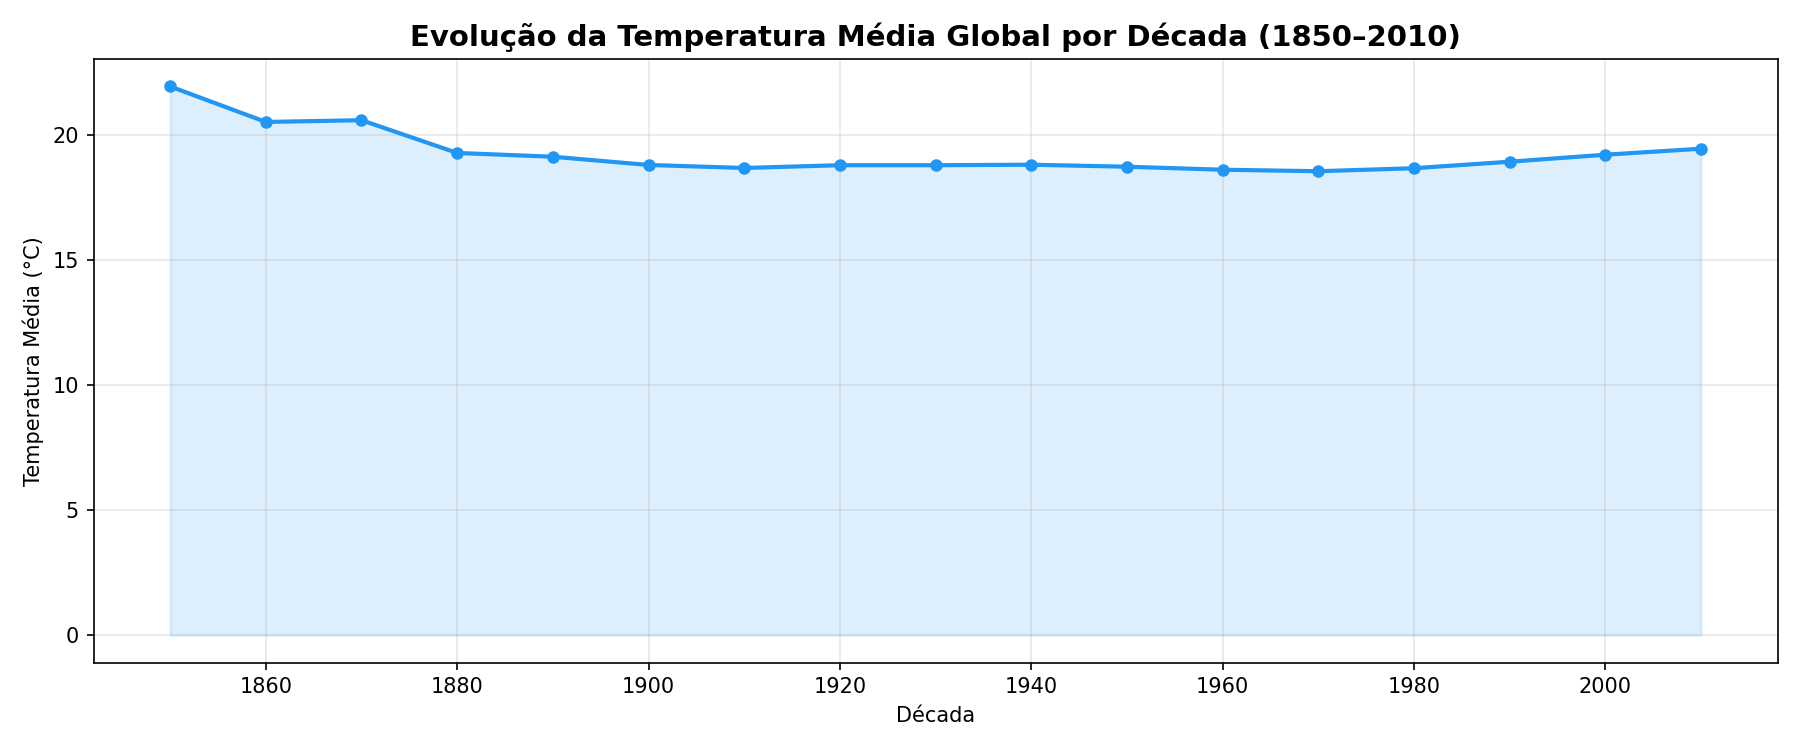
\includegraphics[width=0.85\textwidth]{../spark-data/output/grafico_p1_temperatura_decadas.png}
  \caption{Evolução da temperatura média global por década.}
  \label{fig:p1}
\end{figure}

\textbf{Interpretação:} o aquecimento mais pronunciado concentra-se nas décadas finais:
entre 1980 (18,67\,°C) e 2010 (19,45\,°C) há um aumento de $\sim$\textbf{0,78\,°C}, e a
curva sobe de forma consistente de 1980 em diante. As décadas intermediárias (1950, 1980)
chegam a ficar ligeiramente \textbf{abaixo} de 1900, o que não indica resfriamento real,
mas sim o \textbf{viés de composição} do \textit{dataset}: o conjunto de cidades medidas
muda ao longo do tempo, e a média global é sensível a quais estações estão presentes em
cada década. A aceleração recente é coerente com o aquecimento global documentado na
literatura.

\subsection{P2 --- 10 anos mais quentes por continente}

\textbf{O que foi feito:} restringiram-se os dados aos últimos 50 anos
(\texttt{Year >= 1974}) e agruparam-se os países em \textbf{sete regiões continentais}
(América do Sul, América do Norte, América Central e Caribe, Europa, Ásia, África e
Oceania). Cada região reúne \textbf{praticamente todos os seus países} presentes no
\textit{dataset} da ordem de dezenas por região, e não apenas uma amostra. Para
cada região, calculou-se a temperatura média anual, ordenando de forma decrescente e
tomando o \textit{top}~10.

\begin{lstlisting}[caption={Ranking dos anos mais quentes por região continental.},label={lst:p2}]
continentes = {
    "America do Sul":           ["Brazil", "Argentina", "Chile", "Colombia",
                                  "Peru", "Venezuela", "Ecuador", "Bolivia", ...],
    "America do Norte":         ["United States", "Canada", "Mexico"],
    "America Central e Caribe": ["Guatemala", "Honduras", "Cuba", "Haiti",
                                  "Dominican Republic", "Jamaica", ...],
    "Europa":                   ["Germany", "France", "United Kingdom", "Spain",
                                  "Sweden", "Norway", "Poland", "Ukraine", ...],
    "Asia":                     ["China", "India", "Japan", "Russia", "Iran",
                                  "Turkey", "Saudi Arabia", "Kazakhstan", ...],
    "Africa":                   ["Nigeria", "South Africa", "Egypt", "Kenya",
                                  "Algeria", "Morocco", "Sudan", "Angola", ...],
    "Oceania":                  ["Australia", "New Zealand", "Papua New Guinea"],
}

df_recente = df_filtrado.filter(col("Year") >= 1974)
for continente, paises in continentes.items():
    df_cont = (
        df_recente.filter(col("Country").isin(paises))
        .groupBy("Year")
        .agg(_round(avg("AverageTemperature"), 2).alias("AvgTemp"))
        .orderBy(col("AvgTemp").desc())
        .limit(10)
    )
    df_cont.show()
\end{lstlisting}

\textbf{Resultado} (3 anos mais quentes e pico de temperatura por região):
\begin{itemize}
  \item \textbf{América Central e Caribe:} 1998, 1997, 2003 (pico $\sim 25{,}9$\,°C)
  \item \textbf{África:} 2010, 2005, 1998 (pico $\sim 24{,}4$\,°C)
  \item \textbf{América do Sul:} 1998, 2002, 2012 (pico $\sim 22{,}2$\,°C)
  \item \textbf{Ásia:} 2013, 2010, 2012 (pico $\sim 22{,}1$\,°C)
  \item \textbf{América do Norte:} 2013, 2012, 1998 (pico $\sim 17{,}5$\,°C)
  \item \textbf{Oceania:} 2013, 1998, 2010 (pico $\sim 16{,}9$\,°C)
  \item \textbf{Europa:} 2007, 2011, 2013 (pico $\sim 11{,}5$\,°C)
\end{itemize}

\textbf{Interpretação:} os anos mais quentes concentram-se majoritariamente após 1998,
reforçando o aquecimento recente. Anos como \textbf{1998} e \textbf{2013} aparecem no topo
de quase todas as regiões. A ordenação por temperatura absoluta segue a latitude:
\textbf{América Central e Caribe} e \textbf{África} (faixas tropicais) lideram, enquanto
\textbf{Europa} fica por último --- mais fria agora que a lista inclui países nórdicos e do
leste europeu. Note que a média da Europa caiu em relação a uma amostra menor de países,
ilustrando como a composição do conjunto afeta o valor absoluto.

\begin{figure}[H]
  \centering
  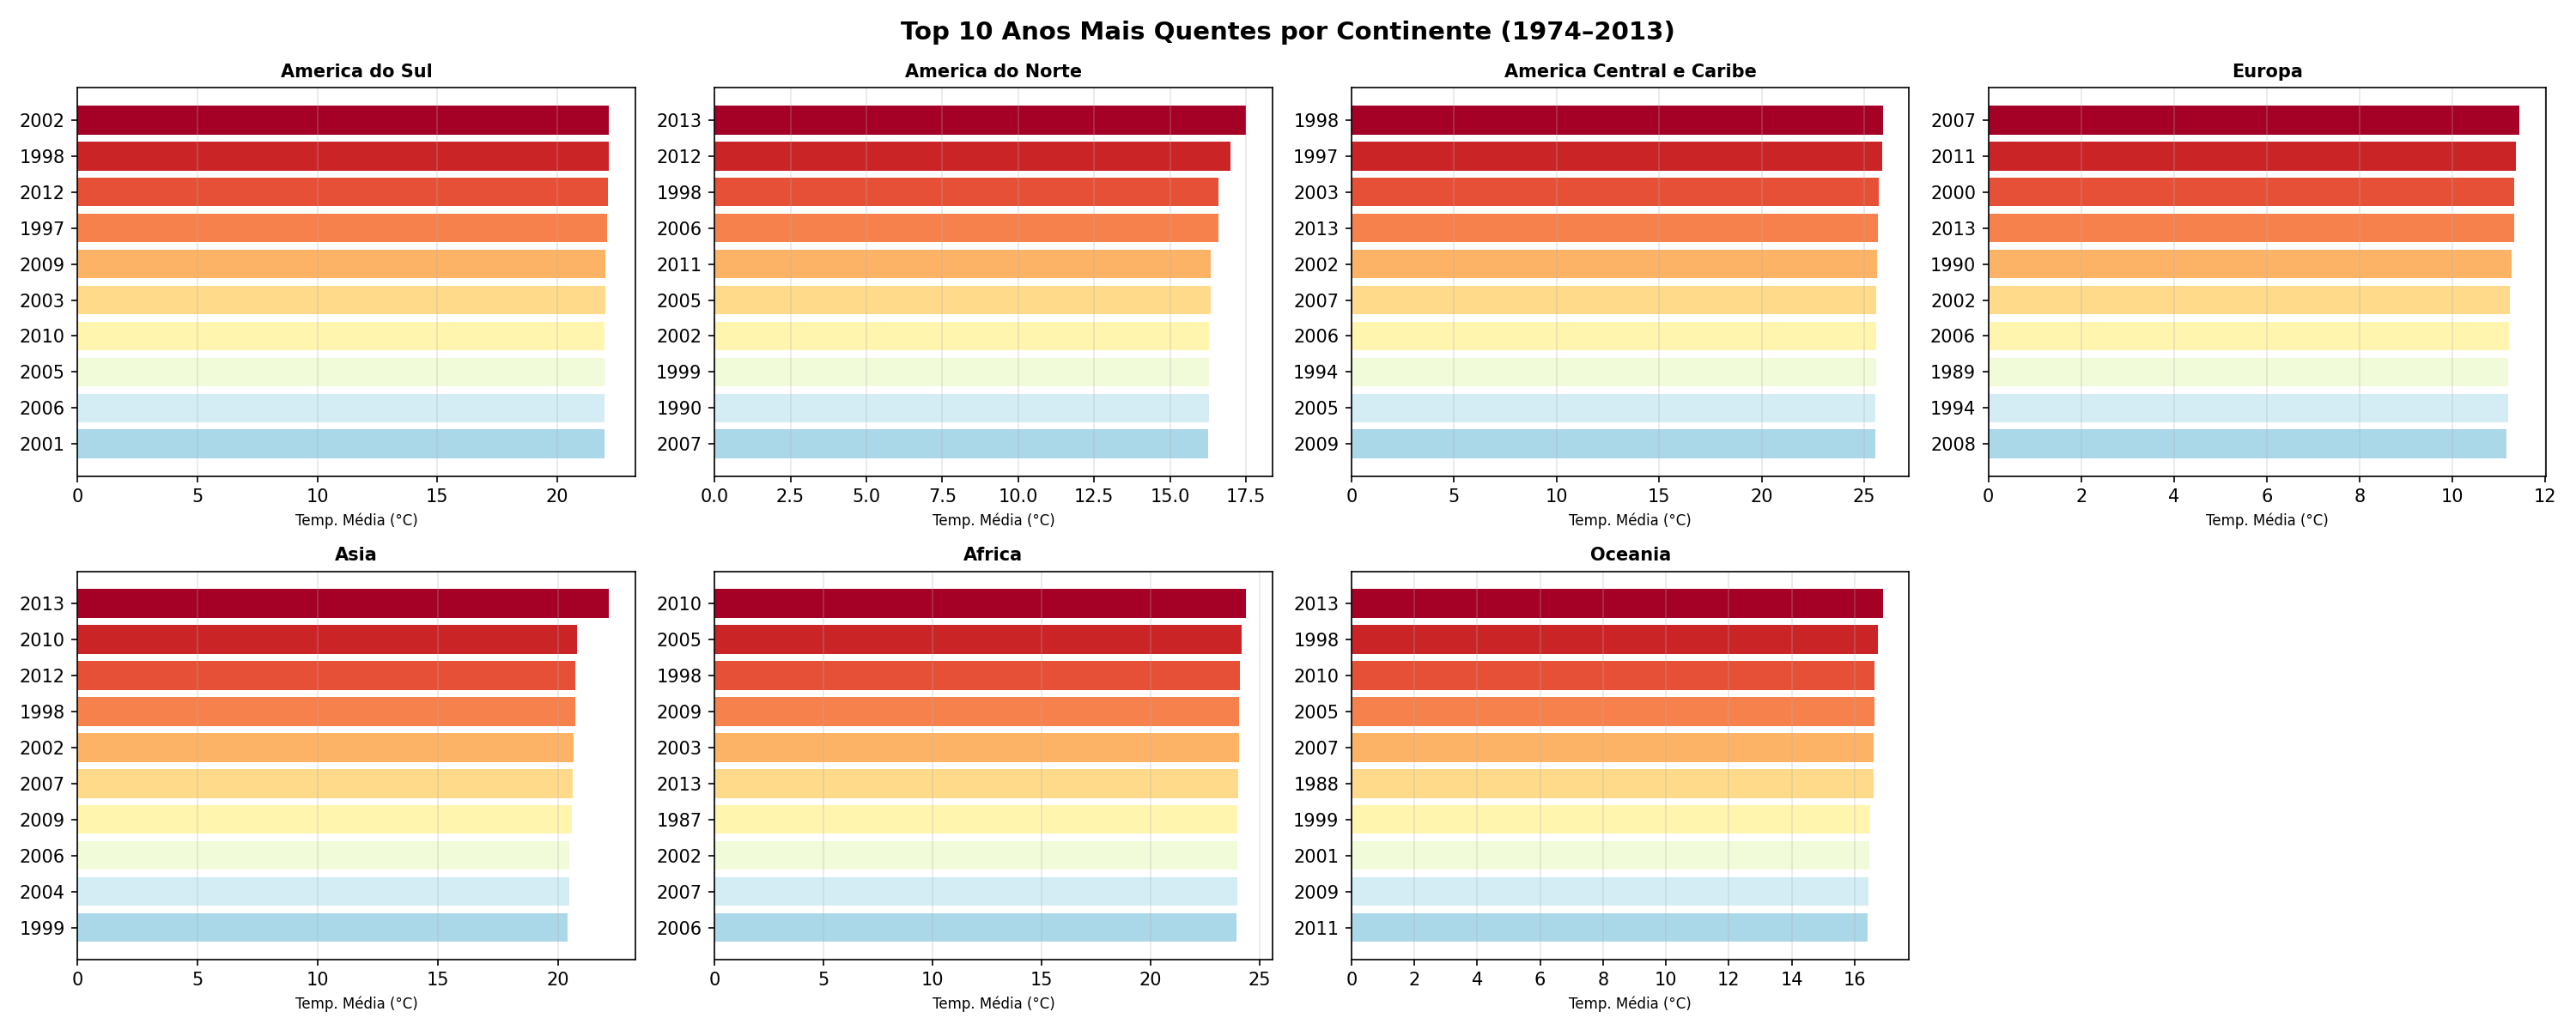
\includegraphics[width=0.95\textwidth]{../spark-data/output/grafico_p2_anos_quentes_continente.png}
  \caption{Top 10 anos mais quentes por continente (1974--2013).}
  \label{fig:p2}
\end{figure}

\textbf{Limitação metodológica:} o \textit{dataset} não possui uma coluna de continente; o
agrupamento por região foi montado manualmente. Embora agora abranja a quase totalidade
dos países de cada região (tornando as médias bem mais representativas que um recorte
pequeno), permanecem dois vieses: países sem registros no \textit{dataset} não entram, e a
média é simples por país/ano --- não ponderada por área ou número de estações.

\subsection{P3 --- Cidades em risco (maior instabilidade)}

\textbf{O que foi feito:} considerando o último século (\texttt{Year >= 1920}),
agruparam-se os dados por cidade/país e calculou-se o \textbf{desvio padrão} da
temperatura, indicador de volatilidade climática. O \textit{top}~10 representa as cidades
de clima mais instável.

\begin{lstlisting}[caption={Cidades com maior desvio padrão de temperatura.},label={lst:p3}]
df_risk = (
    df_filtrado.filter(col("Year") >= 1920)
    .groupBy("City", "Country")
    .agg(_round(stddev("AverageTemperature"), 2).alias("Temperature_StdDev"))
    .orderBy(col("Temperature_StdDev").desc())
    .limit(10)
)
df_risk.show()
\end{lstlisting}

\textbf{Resultado:} a cidade de maior instabilidade é \textbf{Yichun (China)}, com desvio
padrão de \textbf{14,34\,°C}. As dez primeiras colocadas são todas cidades do
\textbf{nordeste da China}.

\begin{figure}[H]
  \centering
  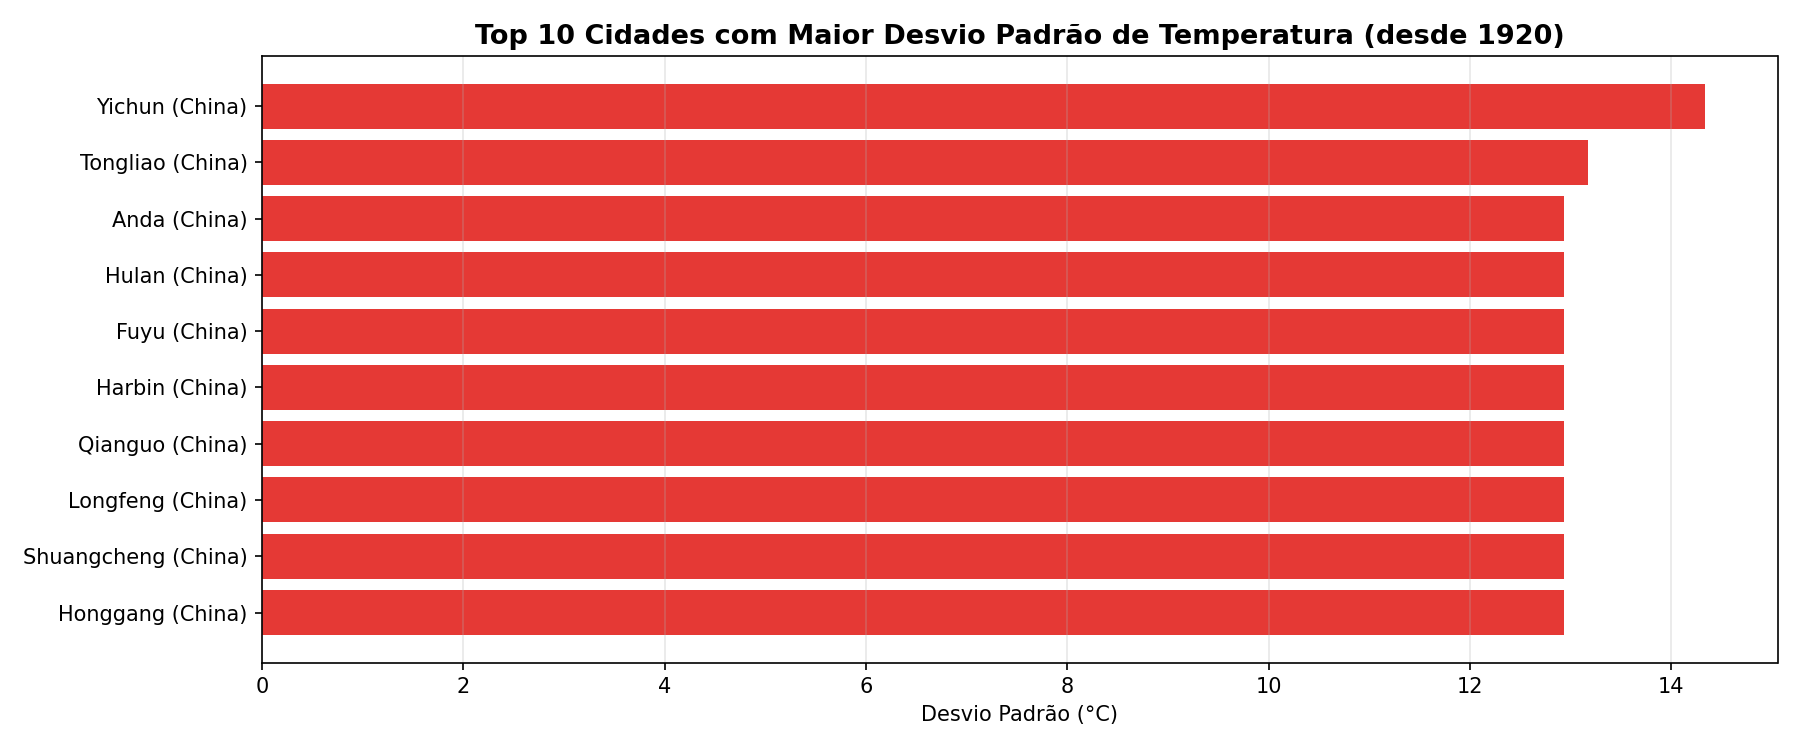
\includegraphics[width=0.85\textwidth]{../spark-data/output/grafico_p3_cidades_risco.png}
  \caption{Top 10 cidades com maior desvio padrão de temperatura.}
  \label{fig:p3}
\end{figure}

\textbf{Interpretação:} o domínio de cidades do nordeste chinês reflete o
\textbf{clima continental extremo} da região, caracterizado por invernos rigorosos e
verões quentes, o que produz amplitudes térmicas anuais muito elevadas.

\subsection{P4 --- Correlação entre máximas e mínimas nos trópicos}

\textbf{O que foi feito:} filtraram-se as cidades na faixa tropical
(\texttt{Latitude} entre $-23{,}5$ e $23{,}5$) e, por cidade/ano, calcularam-se a
temperatura máxima (\texttt{T\_Max}) e mínima (\texttt{T\_Min}) mensais. Em seguida,
mediu-se o coeficiente de correlação de Pearson entre elas com \texttt{stat.corr}.

\begin{lstlisting}[caption={Correlação entre T\_Max e T\_Min nas zonas tropicais.},label={lst:p4}]
df_tropicos = (
    df_filtrado.filter((col("Latitude") >= -23.5) & (col("Latitude") <= 23.5))
    .groupBy("City", "Year")
    .agg(
        _max("AverageTemperature").alias("T_Max"),
        _min("AverageTemperature").alias("T_Min"),
    )
)
corr_t = df_tropicos.stat.corr("T_Max", "T_Min")
\end{lstlisting}

\textbf{Resultado:} coeficiente de Pearson de \textbf{0,4026}.

\begin{figure}[H]
  \centering
  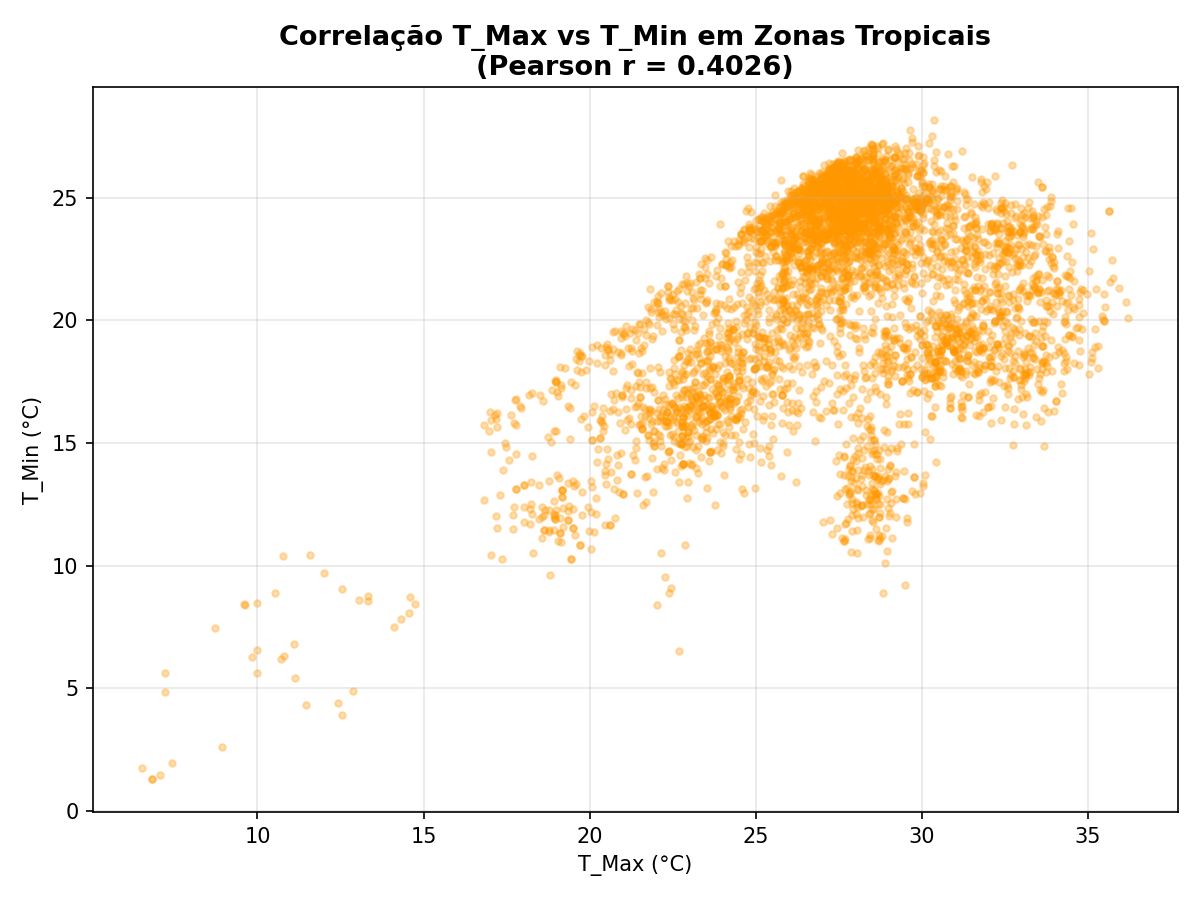
\includegraphics[width=0.85\textwidth]{../spark-data/output/grafico_p4_correlacao_tropicais.png}
  \caption{Dispersão entre temperaturas máximas e mínimas nas zonas tropicais.}
  \label{fig:p4}
\end{figure}

\textbf{Interpretação:} há uma correlação \textbf{moderada positiva} entre máximas e
mínimas. Faz sentido nos trópicos: anos mais quentes tendem a elevar tanto as máximas
quanto as mínimas, mas a correlação não é forte porque outros fatores (umidade,
sazonalidade, altitude) também influenciam.

\subsection{P5 --- Qualidade dos dados}

\textbf{O que foi feito:} usando a média histórica por cidade,
removeram-se os registros cuja \texttt{AverageTemperatureUncertainty} excedia 10\% da
média da cidade, e agruparam-se os removidos por país.

\begin{lstlisting}[caption={Registros de alta incerteza removidos, agrupados por país.},label={lst:p5}]
df_alta_incerteza = df_limpo_com_histavg.filter(
    col("AverageTemperatureUncertainty") > (0.10 * col("HistAvg"))
)
df_alta_incerteza.groupBy("Country").count().orderBy(col("count").desc()).show(10)
\end{lstlisting}

\textbf{Resultado:} os países com mais registros descartados foram
\textbf{Rússia} (344.520), \textbf{China} (256.988) e \textbf{EUA} (191.539). Ao todo,
cerca de \textbf{1.938.936} registros foram removidos --- o conjunto passou de
\textbf{8.235.082} para \textbf{6.296.146} linhas.

\textbf{Interpretação:} a concentração de descartes em países de grande extensão
territorial e com séries históricas mais antigas é esperada: medições remotas e
instrumentos antigos carregam maior incerteza. O filtro removeu $\sim 23{,}5\%$ dos
dados, melhorando a confiabilidade das análises seguintes ao custo de algum volume.

\subsection{P6 --- Correlação entre emissões de CO\textsubscript{2} e aquecimento}

A pergunta do enunciado é precisa: existe correlação entre o \textbf{aumento das emissões}
de CO\textsubscript{2} de um país e o \textbf{aumento da sua temperatura} nos últimos 50
anos? A palavra-chave é \textit{aumento} --- trata-se de correlacionar \textbf{tendências}
(variação ao longo do tempo), e não níveis absolutos. Por isso a questão foi abordada em
duas etapas.

\subsubsection{Etapa 1 --- Cruzamento das bases (\textit{join})}

Primeiro agregou-se a temperatura média por país/ano (últimos 50 anos) e fez-se um
\textbf{\textit{inner join}} com a base de CO\textsubscript{2} limpa pelas chaves país e
ano, conforme exigido pelo desafio. Uma correlação ingênua sobre os \textbf{níveis
absolutos} serve apenas como diagnóstico inicial.

\begin{lstlisting}[caption={Join entre temperatura e emissões; correlação de níveis (diagnóstico).},label={lst:p6a}]
df_temp_country = (
    df_filtrado.filter(col("Year") >= 1974)
    .groupBy("Country", "Year")
    .agg(avg("AverageTemperature").alias("AvgTemp"))
)

df_join = df_temp_country.join(
    df_co2_clean,
    (df_temp_country["Country"] == df_co2_clean["Country_CO2"])
    & (df_temp_country["Year"] == df_co2_clean["Year_CO2"]),
    "inner",
).dropna(subset=["co2", "AvgTemp"])

corr_nivel = df_join.stat.corr("co2", "AvgTemp")   # -0.1727
\end{lstlisting}

\textbf{Resultado da Etapa 1:} Pearson de \textbf{$-0{,}1727$} sobre o \textit{join} de
\textbf{5.829} registros. Esse valor é \textbf{enganoso}: correlacionar emissão absoluta
com a temperatura \textit{média} do país sofre de \textbf{viés de confundimento
geográfico} --- grandes emissores como Rússia e Canadá são países frios, então a latitude
domina o sinal. Esse número \textbf{não responde} à pergunta, que é sobre \textit{aumento}
e não sobre nível.

\begin{figure}[H]
  \centering
  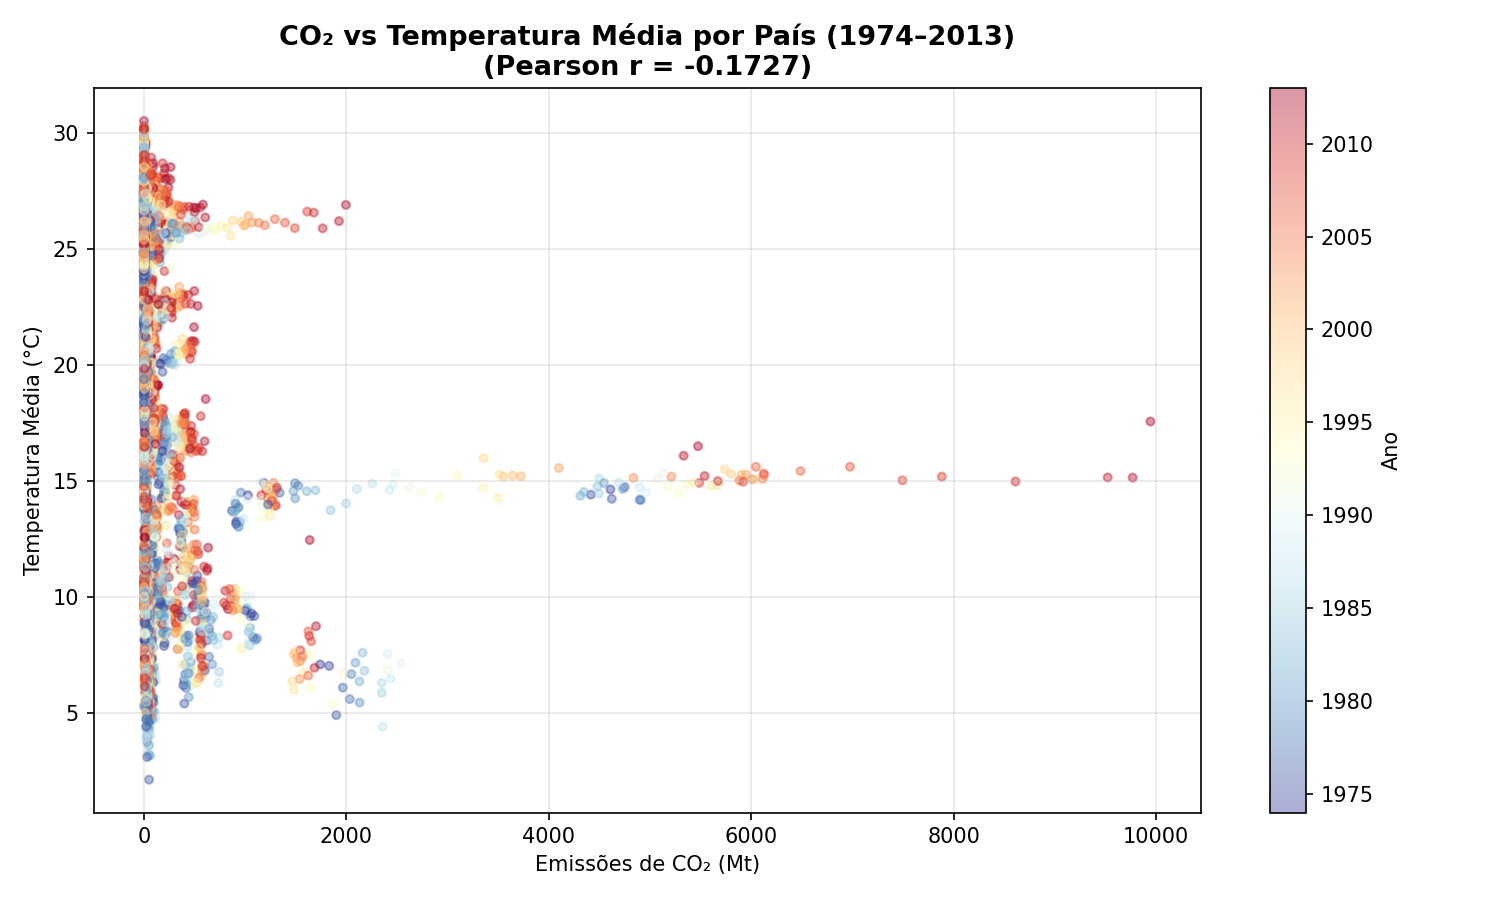
\includegraphics[width=0.78\textwidth]{../spark-data/output/grafico_p6_co2_temperatura.png}
  \caption{Etapa 1 (diagnóstico): emissão absoluta vs temperatura média por país --- correlação distorcida pela geografia.}
  \label{fig:p6a}
\end{figure}

\subsubsection{Etapa 2 --- Correlação das taxas de aumento (resposta à pergunta)}

Para responder de fato, calculou-se, para \textbf{cada país}, a \textbf{tendência} (taxa de
variação anual) tanto da temperatura quanto das emissões, via inclinação da regressão
linear --- obtida em forma fechada por $\text{slope} = \mathrm{cov}(\text{ano},
x)/\mathrm{var}(\text{ano})$, usando as funções \texttt{covar\_pop} e \texttt{var\_pop}
sobre uma janela por país. Em seguida correlacionaram-se as duas tendências
\textbf{através dos países} (exigindo no mínimo 10 anos de dados por país).

\begin{lstlisting}[caption={Tendência (slope) por país e correlação dos aumentos.},label={lst:p6b}]
from pyspark.sql.functions import covar_pop, var_pop, count

slopes = (
    df_join.groupBy("Country").agg(
        (covar_pop("Year", "AvgTemp") / var_pop("Year")).alias("slope_temp"),
        (covar_pop("Year", "co2") / var_pop("Year")).alias("slope_co2"),
        count("*").alias("n"),
    ).filter(col("n") >= 10)
)

corr_variacao = slopes.stat.corr("slope_temp", "slope_co2")   # -0.0017
\end{lstlisting}

\textbf{Resultado da Etapa 2:} Pearson de \textbf{$-0{,}0017$} entre as taxas de aumento,
sobre \textbf{147 países} --- ou seja, \textbf{correlação praticamente nula}.

\begin{figure}[H]
  \centering
  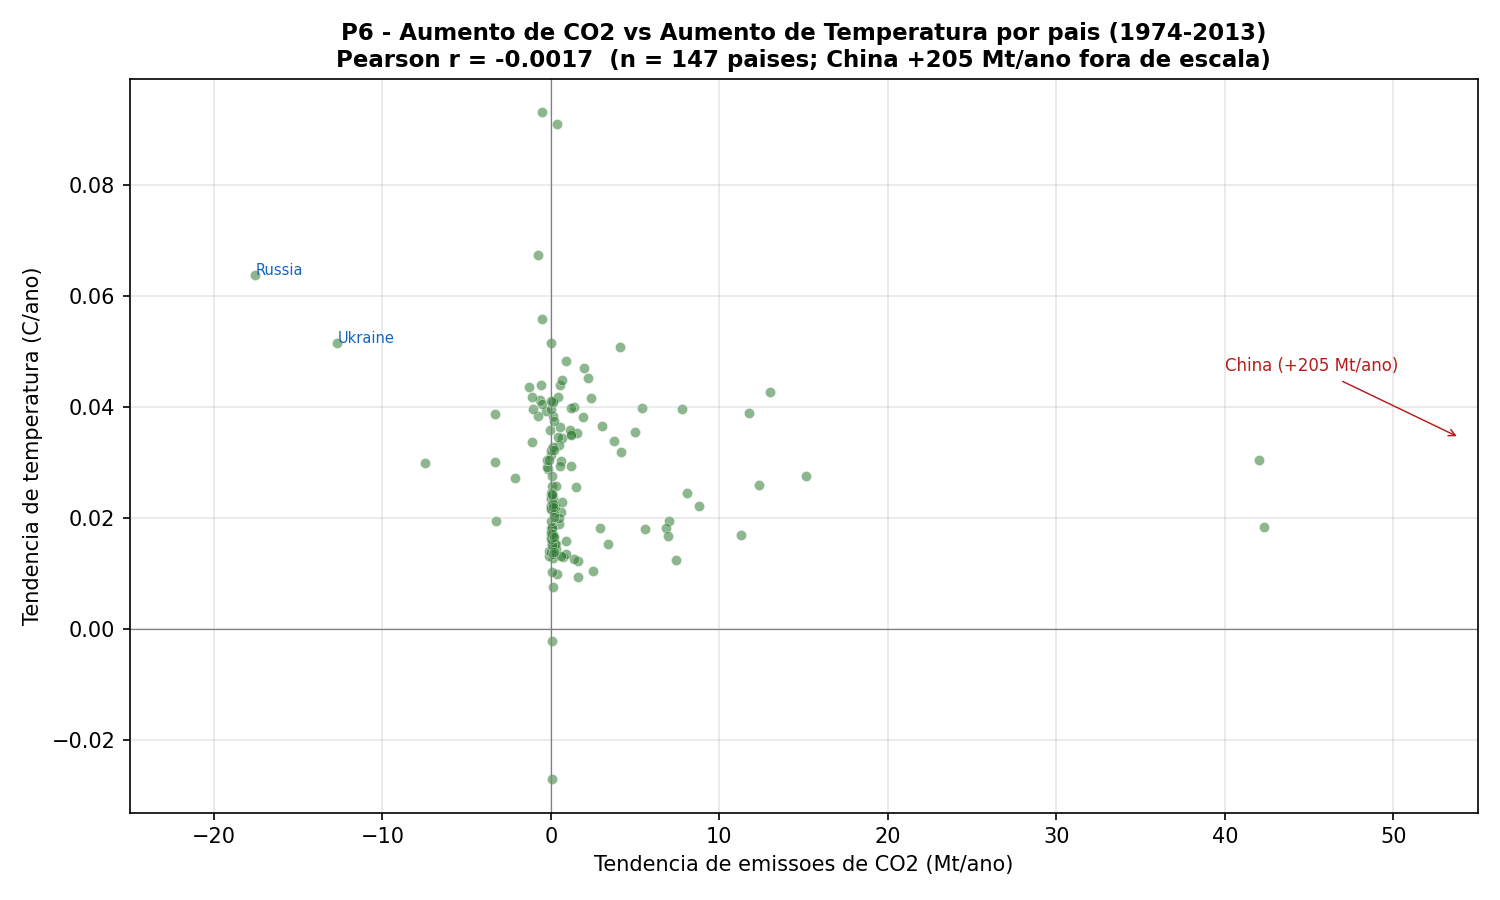
\includegraphics[width=0.85\textwidth]{../spark-data/output/grafico_p6_variacao.png}
  \caption{Etapa 2 (resposta): tendência de emissões vs tendência de temperatura por país. Quase todos os países aquecem ($y>0$) independentemente da trajetória de emissões.}
  \label{fig:p6b}
\end{figure}

\textbf{Interpretação:} ao nível de país, \textbf{não há correlação linear} entre o quanto
um país aumentou suas emissões e o quanto ele aqueceu. O gráfico deixa isso evidente:
\textbf{quase todos} os países apresentam tendência de temperatura \textbf{positiva}
($+0{,}01$ a $+0{,}09$\,°C/ano), espalhados por toda a faixa de tendências de emissão.
Os casos extremos são ilustrativos: \textbf{Rússia} e \textbf{Ucrânia} aqueceram entre os
mais rápidos do mundo, mas suas emissões \textbf{caíram} ($\sim$$-17$ e $-13$\,Mt/ano)
após o colapso da União Soviética nos anos 1990. Isso é cientificamente coerente: o
CO\textsubscript{2} é um gás \textbf{globalmente bem misturado}, de modo que o aquecimento
de um país é determinado pelo forçamento \textbf{global} (e por efeitos regionais, como a
amplificação ártica), e não pelas suas emissões \textbf{locais}. A resposta honesta à
pergunta, portanto, é que \textbf{não se observa correlação estatística entre o aumento das
emissões de um país e o aumento da sua temperatura} --- e a ausência de correlação é, ela
própria, o achado relevante. Nota: a regressão de Pearson é sensível a \textit{outliers}
como a China ($+205$\,Mt/ano), exibida fora de escala no gráfico.

\subsection{P7 --- Aceleração térmica (\textit{Window Functions})}

\textbf{O que foi feito:} calculou-se a temperatura média por país e década e, com uma
janela particionada por país e ordenada por década, usou-se \texttt{lag} para obter a
temperatura da década anterior. A aceleração é a diferença entre a década de 2010 e a
anterior; ordenou-se de forma decrescente.

\begin{lstlisting}[caption={Aceleração térmica por país via lag em Window Function.},label={lst:p7}]
df_decada_pais = (
    df_filtrado.withColumn("Decada", (col("Year") / 10).cast("int") * 10)
    .groupBy("Country", "Decada")
    .agg(avg("AverageTemperature").alias("TempDecada"))
)

window_accel = Window.partitionBy("Country").orderBy("Decada")
df_accel = (
    df_decada_pais.withColumn("TempAnterior", lag("TempDecada", 1).over(window_accel))
    .withColumn("Aceleracao", col("TempDecada") - col("TempAnterior"))
    .filter(col("Decada") == 2010)
    .orderBy(col("Aceleracao").desc())
    .limit(10)
)
\end{lstlisting}

\textbf{Resultado (aceleração em °C entre a década de 2010 e a anterior):}
\begin{itemize}
  \item Finlândia (1,076), Rússia (1,049), Cazaquistão (0,778), Canadá (0,767)
  \item Irã (0,761), Iraque (0,736), Geórgia (0,727), Armênia (0,727)
  \item Turquia (0,663), Tajiquistão (0,639)
\end{itemize}

\begin{figure}[H]
  \centering
  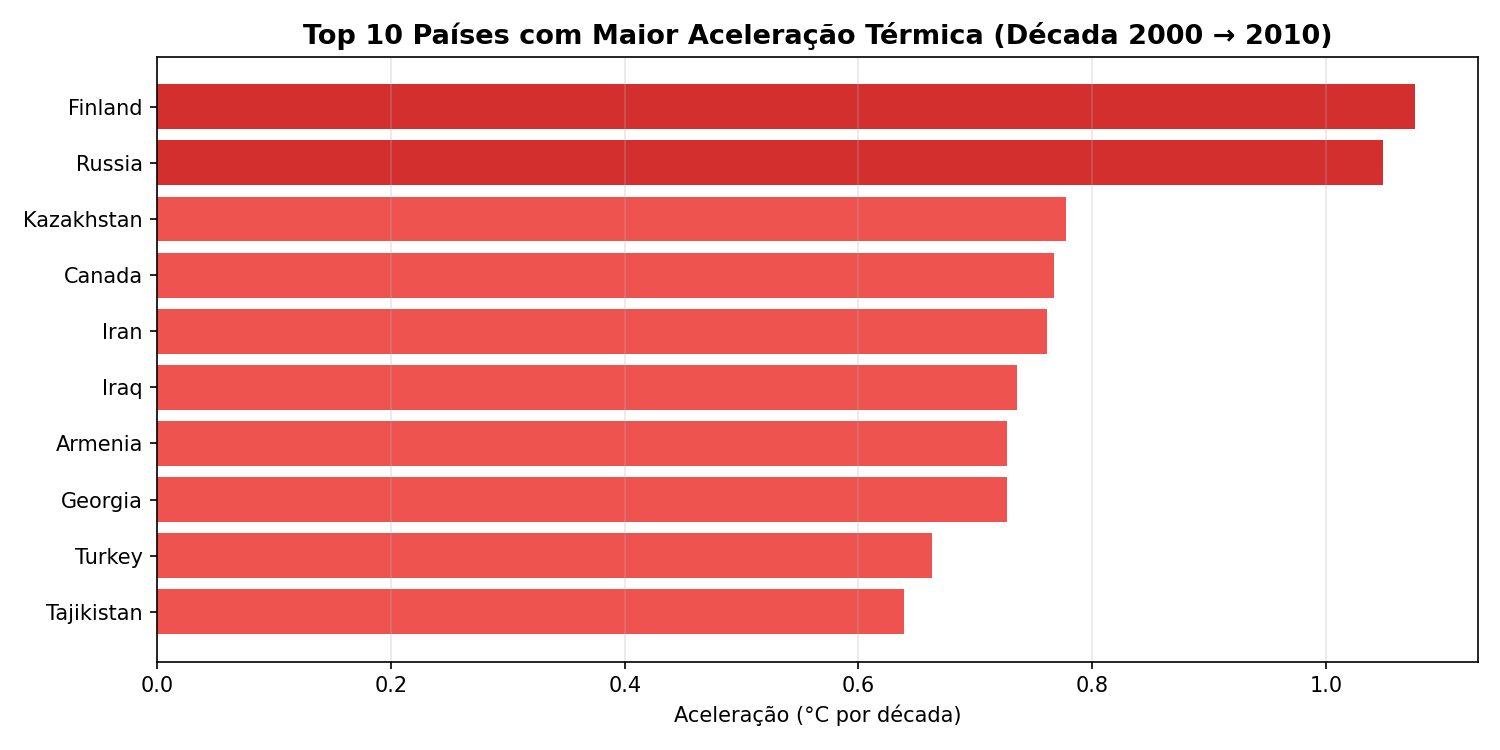
\includegraphics[width=0.85\textwidth]{../spark-data/output/grafico_p7_aceleracao_termica.png}
  \caption{Top 10 países com maior aceleração térmica.}
  \label{fig:p7}
\end{figure}

\textbf{Interpretação:} predominam países de \textbf{altas latitudes do hemisfério norte}
(Finlândia, Rússia, Canadá) e do \textbf{Oriente Médio/Cáucaso}. O resultado é consistente
com o fenômeno da \textbf{amplificação do Ártico}, em que regiões setentrionais aquecem
mais rápido que a média global. Note que esta análise por \textit{variação} (P7) é mais
robusta que a correlação por níveis absolutos da P6.

\subsection{P8 --- Previsão de temperatura com MLlib}

\textbf{O que foi feito:} para a cidade de São Paulo (1993--2013), montou-se um conjunto
de treino com a temperatura média anual. Usando \texttt{VectorAssembler} (transformando o
ano em vetor de \textit{features}) e \texttt{LinearRegression} do Spark MLlib, treinou-se
um modelo e previram-se os anos de 2014 a 2018.

\begin{lstlisting}[caption={Regressão linear para previsão de temperatura em São Paulo.},label={lst:p8}]
df_sp = (
    df_filtrado.filter((col("City") == "São Paulo") & (col("Year") >= 1993))
    .groupBy("Year")
    .agg(avg("AverageTemperature").alias("label"))
    .orderBy("Year")
)

assembler = VectorAssembler(inputCols=["Year"], outputCol="features")
df_ml = assembler.transform(df_sp).select("features", "label")

lr = LinearRegression(featuresCol="features", labelCol="label")
lr_model = lr.fit(df_ml)

anos_futuros = spark.createDataFrame([(y,) for y in range(2014, 2019)], ["Year"])
previsoes = lr_model.transform(assembler.transform(anos_futuros))
\end{lstlisting}

\textbf{Resultado:} coeficiente de \textbf{$-0{,}000099$} e intercepto de \textbf{20,79},
gerando previsão de $\sim$\textbf{20,59\,°C} para 2014--2018.

\begin{figure}[H]
  \centering
  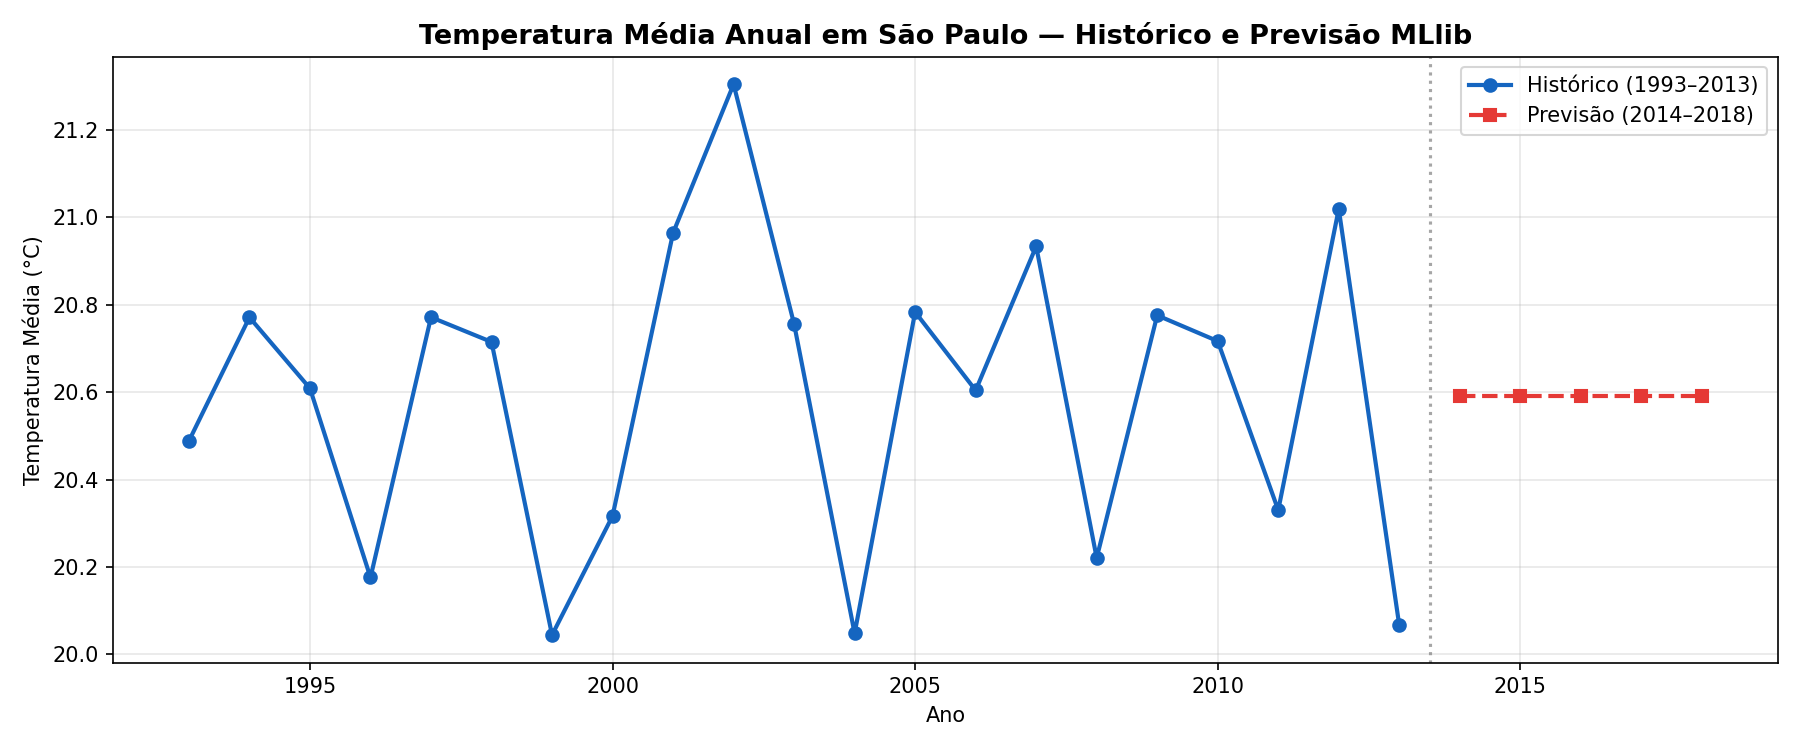
\includegraphics[width=0.85\textwidth]{../spark-data/output/grafico_p8_previsao_saopaulo.png}
  \caption{Temperatura histórica e previsão linear para São Paulo.}
  \label{fig:p8}
\end{figure}

\textbf{Interpretação:} o coeficiente angular praticamente nulo indica uma tendência
\textbf{estável} no período analisado para São Paulo. É importante reconhecer as
\textbf{limitações}: o modelo é linear e simples, treinado com poucas amostras anuais
($\sim$21 pontos), o que o torna sensível a ruído e inadequado para extrapolações de longo
prazo. Serve como demonstração da integração do MLlib ao pipeline, não como projeção
climática rigorosa.

\section{Evidências do Spark UI}
\label{sec:sparkui}

O monitoramento das execuções foi feito pela \textbf{Spark UI} (porta \texttt{8080} no
master) e pelo \textbf{History Server} (porta \texttt{18080}), que preserva o histórico de
aplicações concluídas. Os números a seguir foram \textbf{extraídos do log de eventos da
execução real} da aplicação \texttt{AnaliseClimaticaGlobal} --- a mesma que gerou os
gráficos deste relatório ---, cujo \textit{pipeline} completo levou
$\sim$\textbf{1\,min\,43\,s}. As capturas de tela correspondentes devem ser inseridas
manualmente pelo autor; os pontos a destacar em cada uma estão descritos abaixo.

\subsection{DAG das operações mais pesadas}

As operações de maior custo, identificadas pela aba \textbf{Stages}, são:
\begin{itemize}
  \item \textbf{Leitura e materialização da base (532\,MB):} a ingestão do CSV e a
        primeira contagem disparam estágios com \textbf{6 tarefas} (uma por core do
        cluster), que concentram o maior peso de E/S do \textit{pipeline}
        ($\sim$10\,s de leitura e $\sim$13\,s na contagem que materializa o cache).
  \item \textbf{P5 --- \textit{Window Function}:} o cálculo da média histórica
        particionada por \texttt{City}/\texttt{Country} exige um \textbf{\textit{shuffle}}
        (operador \texttt{Exchange}) para reorganizar os dados por chave. Mediu-se um
        \textit{shuffle} de $\sim$\textbf{105\,MB} entre os estágios de escrita e leitura
        (a etapa P5 completa levou $\sim$9\,s).
  \item \textbf{P6 --- \textit{Join}:} o \textit{inner join} por país/ano provoca
        \textit{shuffle} de ambos os lados, confirmado no log como um
        \texttt{SortMergeJoin} (\textit{shuffle} de $\sim$\textbf{134\,MB}, e não um
        \textit{broadcast}); a etapa P6 completa levou $\sim$9\,s.
\end{itemize}

\subsection{Estágios, tempo de execução e tarefas}

A execução analisada gerou \textbf{quase duas centenas de estágios} (numerados até
$\sim$187), dos quais muitos aparecem como \texttt{SKIPPED} --- efeito da reutilização de
resultados (\textit{stage reuse}) e do \textit{cache}. Pontos a comentar nas capturas:
\begin{itemize}
  \item \textbf{Número de tarefas por estágio:} os estágios de leitura e agregação
        executam com \textbf{6 tarefas}, refletindo os \textbf{6 cores} dos 3 workers.
        Embora o valor lógico de \texttt{spark.sql.shuffle.partitions} seja 200, o
        \textbf{\textit{Adaptive Query Execution} (AQE)} --- ativo por padrão no Spark
        3.5 --- \textit{coalesce} as partições pós-\textit{shuffle} para apenas
        \textbf{6 a 7 tarefas}, pois o volume de dados após as agregações é pequeno.
        É esse valor reduzido (e não 200) que se observa na UI.
  \item \textbf{Tempo de execução e paralelismo:} a distribuição das tarefas entre os
        \textbf{3 workers} (6 cores no total) é visível na aba \textbf{Executors},
        demonstrando o paralelismo efetivo do cluster.
  \item \textbf{\textit{Shuffles} repetidos:} observam-se vários estágios reescrevendo
        $\sim$128\,MB de \textit{shuffle} (a agregação \texttt{df\_temp\_country} de P6)
        recomputados a cada ação. Isso ocorre porque o \texttt{cache} foi aplicado a
        \texttt{df\_limpo}, e não aos DataFrames já agregados/filtrados --- uma
        oportunidade de otimização adicional.
  \item \textbf{Efeito do \texttt{cache}:} na aba \textbf{Storage}, o DataFrame
        \texttt{df\_limpo} aparece como persistido em memória, confirmando a otimização
        discutida na Seção~\ref{sec:cache}.
\end{itemize}

\begin{figure}[H]
  \centering
  \includegraphics[width=0.9\textwidth]{spark_ui_workers.png}
  \caption{Spark Master UI (\texttt{localhost:8080}) com os 3 workers ativos.}
\end{figure}

\begin{figure}[H]
  \centering
  \includegraphics[width=0.9\textwidth]{spark_ui_jobs.png}
  \caption{Aba Jobs da Spark UI durante a execução do pipeline.}
\end{figure}

\begin{figure}[H]
  \centering
  \includegraphics[width=0.9\textwidth]{spark_ui_dag.png}
  \caption{DAG do stage mais pesado na Spark UI.}
\end{figure}

\begin{figure}[H]
  \centering
  \includegraphics[width=0.9\textwidth]{spark_ui_stages.png}
  \caption{Aba Stages: distribuição de tarefas entre os executors.}
\end{figure}

\begin{figure}[H]
  \centering
  \includegraphics[width=0.9\textwidth]{spark_ui_storage.png}
  \caption{Aba Storage: \texttt{df\_limpo} persistido em memória pelo \texttt{cache()}.}
\end{figure}

\begin{figure}[H]
  \centering
  \includegraphics[width=0.9\textwidth]{spark_ui_executors.png}
  \caption{Aba Executors: 3 workers com tasks distribuídas.}
\end{figure}

% Espaco reservado para as capturas de tela da Spark UI:
% \begin{figure}[H]
%   \centering
%   \includegraphics[width=0.9\textwidth]{caminho/para/print_dag_p5.png}
%   \caption{DAG da Window Function (P5) na Spark UI.}
% \end{figure}
